% ================
% Landon Buell
% Qioayan Yu
% 
% 24 June 2020
% ================

\documentclass[12pt,letterpaper]{article}

\usepackage{float}
\usepackage{graphicx}
\usepackage{subfigure}
\usepackage{amsmath}
\usepackage{amssymb}
\usepackage[left=2.5cm,right=2.5cm,top=2.5cm]{geometry}

\begin{document}


% ================================================================

\section*{Experiment}

\paragraph*{}This case study serves as an experiment in determining how approximate computation techniques may change the performance of a Convolutional Neural Network(CNN)classifier. We have chosen to the the CiFar-10 data set containing 32 x 32 x 3 pixel RGB images of various animals and vehicles. Each pixel is given by an integer $0$ to $255$ (a byte) which encodes the brightness of that pixel. All images are labeled $0$ through $9$, encoding the object that appears with in.
 
\paragraph*{}To apply an approximate computing technique to each image, we use a \textit{mute-bit} function. In doing so, each approximated pixel has gone from being stored as a specific $8$-bit object to $8$-bits of all $0$'s. This is used as a method of approximation to simulate a  This approximation method was applied to exterior pixels of each image sample, to effectively create a border of $N$-approximated pixels in depth. Models with $N = 2,4,6,8$ were compared to an unaffected baseline model. Examples of this approximation can be seen in fig. (\ref{images}).

\begin{figure}[h]
\label{images}
IMAGES!
\end{figure}

\paragraph*{}As a way to compensate for the previously described approximate computing technique, we also explore a method of attempting to recover the information in the lost pixel border. We do this by using sets of the unchanged pixels from the center of the image and copy and pasting them to the outside of the image. In doing this, the previous $N$-pixel border of muted bits is now replaced with features remaining. Thus, key feature that were preserved in the image's center have been duplicated to the previously muted bits on the outside. This can also be seen in fig. (\ref{images}).

\paragraph*{}To test how this method works over different model architecture variants, we use an system inspired from the $VGG-16$ CNN model. This model uses groups of layers that work together to produce feature maps which then pass that map on the next set of layers. We define a \textit{layer group} to be three immediately adjacent layers in a CNN where the first two layers are 2D convolution layers with identical number of output filters and kernel sizes followed by a Max-Pooling layer or and Average Pooling layer. The output of that layer can be fed into another similar layer group or a set of flattening and sense layers moving directly to output. A visual graph of this layer group can be seen in fig. (\ref{Layer Group}).

\begin{figure}[h]
\label{Layer Group}
\begin{center}
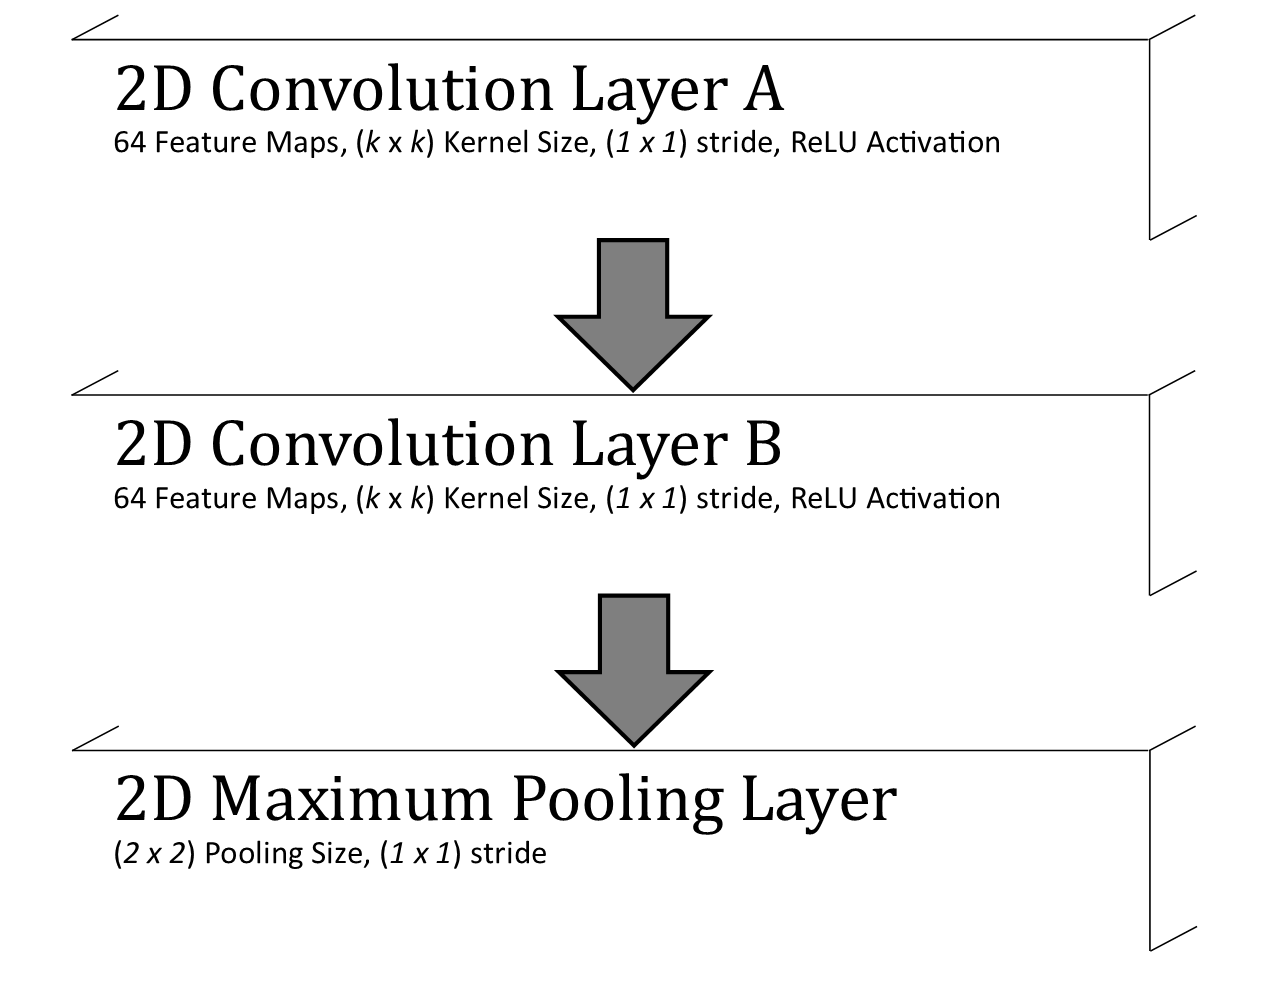
\includegraphics[scale=0.5]{CNN_LayerGroup}
\end{center}
\caption{A graphical representation of the layers that constitute a \textit{Layer Group}. This archtiecture is inspired from the $VGG-16$ model. two Convolution layers work together to produce $64$ feature maps each. The resulting activations are reduced in dimensionality by the maximum pooling layer.}
\end{figure}

\paragraph*{}We test models with one and two layer groups, with kernel sizes $k = 2,3,4,5,6$ for each number of layers. We have set each convolution layer to produce $64$ feature maps, a bias vector, a ($1 x 1$) stride, with a ReLU activation function. Each maximum pooling layer extracts the maximum activation from a ($2 x 2$) block of samples and passed it forward to the next layer. After the Layer Groups have been passed, the activations are reshaped into column vector and passed into a $128$-unit dense ReLU layer, and then a $10$-unit dense softmax output layer.




% ================================================================

\begin{figure}[H]
\label{results}
RESULTS!
\end{figure}

\section*{Conclusion}To mean any changes in performances of the neural-network classifier, we track the  (1) average validation loss value, (2) average validation precision score and (3) average validation recall scores across all $10$ classes.




% ================================================================

\end{document}